\pagestyle{simu}
\addcontentsline{toc}{chapter}{Simulado 1}
\markboth{Simulado 1}{}

\num{1} Leia o texto.

\begin{quote}
\textbf{Novo método de reciclagem pode viabilizar a economia circular dos plásticos}

Resíduos plásticos se espalham aceleradamente pelo planeta causando
danos à biodiversidade, à saúde humana, à economia, e ao equilíbrio
climático. Diante desse desafio crescente, um método inovador –
descrito, em outubro, num artigo publicado pela revista Science –
aponta um promissor caminho de desenvolvimento tecnológico. A abordagem
combina processos biológicos e químicos para simplificar e aumentar a
eficiência da reciclagem de misturas de vários tipos de plástico.

{[}...{]}.

\fonte{Flavio Lobo. IPEA. Novo método de reciclagem pode viabilizar a economia circular dos plásticos. Disponível em: \emph{https://www.ipea.gov.br/cts/pt/central-de-conteudo/noticias/noticias/329-novo-metodo-de-reciclagem-pode-viabilizar-a-economia-circular-dos-plasticos}.
Acesso em: 25 fev. 2023.}
\end{quote}

De acordo com o texto, a nova forma de reciclagem

\begin{minipage}{.5\textwidth}
\begin{escolha}
\item pode ser utilizada só com papel.

\item não é muito prática.

\item aumenta a eficiência do processo.

\item produz maiores quantidades de lixo.
\end{escolha}
\end{minipage}
\sidetext{SAEB: Localizar informação explícita. BNCC: EF15LP03 – Localizar
informações explícitas em textos.}

\num{2} Leia o texto, trecho de um conto de fadas.

\begin{quote}
\textbf{João e o pé de feijão}

Era uma vez garoto chamado João, que morava com sua mãe em uma pequena
casa na floresta. João e sua mãe eram muito pobres e tinham dificuldades
para conseguir dinheiro e comida suficientes para sobreviver.

Um dia, João foi até a cidade para vender a única vaca da família. No
caminho, ele encontrou um homem misterioso que lhe ofereceu cinco
feijões mágicos em troca da vaca. João aceitou e voltou para casa com os
feijões
\fonte{Texto escrito para este material.}
\end{quote}

\pagebreak
Nesse trecho da narrativa, os personagens citados são

\begin{minipage}{.5\textwidth}
\begin{escolha}
\item João, sua mãe e o homem misterioso.

\item João e sua mãe.

\item João e a vaca.

\item João e os feijões.
\end{escolha}
\end{minipage}
\sidetext{SAEB: Identificar elementos constitutivos de textos narrativos. BNCC:
EF35LP26 – Ler e compreender, com certa autonomia, narrativas ficcionais
que apresentem cenários e personagens, observando os elementos da
estrutura narrativa: enredo, tempo, espaço, personagens, narrador e a
construção do discurso indireto e discurso direto.}

\num{3} Leia o texto.

\begin{quote}
\textbf{Brasil terá programa nacional para produção de alimentos saudáveis}\\
\textit{Secretária executiva do MDA falou em evento da Fiocruz, no Rio}

O Ministério do Desenvolvimento Agrário lançará {[}...{]} um programa nacional voltado para estimular a produção de alimentos saudáveis. Segundo a secretária executiva da pasta, Fernanda Machiaveli, a política deve ser anunciada junto com a apresentação do Plano Safra {[}...{]}.

“O programa terá uma visão de estímulo à produção de um alimento saudável, que vem da agroecologia, da agricultura familiar, que é produzido de forma sustentável e saudável”, disse Machiaveli, em entrevista à Agência Brasil, durante seminário da Fundação Oswaldo Cruz (Fiocruz), no Rio de Janeiro. A agroecologia é o conceito que envolve a produção de alimentos saudáveis com respeito a aspectos ambientais, sociais e culturais.

Fernanda explica que, nos últimos anos, tem se observado a redução da diversificação dos alimentos na agricultura familiar com estímulos, por exemplo, à produção de soja por esse segmento.

De acordo com a secretária executiva, uma das frentes do programa será o desestímulo ao uso de agrotóxicos no país. “Essa também é uma agenda que a sociedade civil tem nos demandado”.

{[}...{]}.

\fonte{Vitor Abdala. Agência Brasil. Brasil terá programa nacional para produção de alimentos saudáveis. Disponível em:
\emph{https://brasil.elpais.com/ciencia/2021-12-03/vulcao-das-canarias-abre-caminho-para-a-previsao-das-erupcoes.html}.
Acesso em: 25 fev. 2023.}
\end{quote}

O trecho inicial da notícia, reproduzido aqui, conta com

\begin{escolha}
\item uma imagem ilustrativa, que demonstra visualmente o assunto do texto.

\item um lide, que resume as principais informações da notícia.

\item um subtítulo, que apresenta uma informação não contida no corpo da notícia.

\item um título, que não esclarece o assunto do texto.
\end{escolha}

\coment{SAEB: Analisar elementos constitutivos de gêneros textuais diversos.
BNCC: EF35LP16 – Identificar e reproduzir, em notícias, manchetes, lides
e corpo de notícias simples para público infantil e cartas de reclamação
(revista infantil), digitais ou impressos, a formatação e diagramação
específica de cada um desses gêneros, inclusive em suas versões orais.}

\num{4} Leia o texto.

\begin{quote}
\textbf{Controle e prevenção do desmatamento e dos incêndios florestais}

Prevenir e combater o desmatamento ilegal e os incêndios florestais num
país em desenvolvimento e de dimensões continentais como o Brasil não é
uma tarefa fácil. Principalmente na Amazônia Legal, que corresponde a
cerca de 61\% do território nacional e possui um patrimônio ambiental
com enorme potencial econômico, ainda pouco explorado.

{[}...{]}

São necessárias, portanto, medidas positivas que possam influenciar
novas dinâmicas e modelos produtivos sustentáveis como alternativa à
supressão da vegetação nativa, trazendo os diferentes setores da
sociedade para atuar em conjunto no combate ao desmatamento ilegal.

{[}...{]}.

\fonte{Ministério do Meio Ambiente e Mudança do Clima. Controle e prevenção do desmatamento e dos incêndios florestais.
Disponível em: \emph{https://www.gov.br/mma/pt-br/assuntos/servicosambientais/controle-de-desmatamento-e-incendios-florestais}.
Acesso em: 25 fev. 2023.}
\end{quote}

Esse texto procura convencer o leitor

\begin{escolha}
\item da necessidade de se controlarem e prevenirem os incêndios florestais.

\item da necessidade de se expandir o patrimônio natural brasileiro.

\item das belezas da flora brasileira.

\item dos perigos da diminuição do território natural brasileiro.
\end{escolha}

\coment{SAEB: Analisar o uso de recursos de persuasão em textos verbais e/ou
multimodais. BNCC: EF05LP20 – Analisar a validade e força de argumentos
em argumentações sobre produtos de mídia para público infantil (filmes,
desenhos animados, HQs, games etc.), com base em conhecimentos sobre os
mesmos.}

\pagebreak

\num{5} Leia o trecho de um poema.

\begin{verse}
\textbf{Rosa murcha}

Esta rosa desbotada\\
Já tantas vezes beijada,\\
Pálido emblema de amor;\\
É uma folha caída\\
Do livro da minha vida,\\
Um canto imenso de dor!\\
{[}...{]}

\fonte{Casimiro de Abreu. Rosa murcha. In: \emph{As primaveras}.
Rio de Janeiro: Typ. de Paula Brito, 1859.}
\end{verse}

Representando cada rima com uma letra maiúscula, o esquema de rimas dessa estrofe é

\begin{minipage}{.5\textwidth}
\begin{escolha}
\item AABBCC.

\item ABCABC.

\item ABABCC.

\item AABCCB.
\end{escolha}
\end{minipage}
\sidetext{SAEB: Reconhecer diferentes modos de organização composicional de textos em versos.
BNCC: EF35LP27 – Ler e compreender, com certa autonomia,
textos em versos, explorando rimas, sons e jogos de palavras, imagens
poéticas (sentidos figurados) e recursos visuais e sonoros.}

\num{6} Leia o trecho de um texto.

\begin{quote}
Um destes dias, leva por aí algum tiro para lhe botar juízo na
\textbf{cachola} {[}...{]} Nem sempre há de ter cartas de irmão para
sair-se bem da \textbf{rascada}.

\fonte{Visconde de Taunay. Inocência. Disponível:
\emph{http://objdigital.bn.br/Acervo\_Digital/livros\_eletronicos/inocencia.pdf}.
Acesso em: 26 fev. 2023.}
\end{quote}

Os termos destacados também significam, respectivamente

\begin{minipage}{.5\textwidth}
\begin{escolha}
\item cachoeira e rasgo.

\item cabeça e enrascada.

\item caixa e risco.

\item cacho e risco.
\end{escolha}
\end{minipage}
\sidetext{SAEB: Identificar as variedades linguísticas em textos. BNCC: EF35LP22
- Perceber diálogos em textos narrativos, observando o efeito de sentido
de verbos de enunciação e, se for o caso, o uso de variedades
linguísticas no discurso direto.}

\pagebreak

\num{7} Leia o texto.

\begin{quote}
\textbf{Viver mais de 100 anos?}

Foi publicado, nos Estados Unidos, um estudo segundo o qual somente 1 norte-americano,
a cada 5 milhões de pessoas, consegue ultrapassar a barreira dos 110 anos de idade.
O estudo, de longo prazo, é da Universidade de Boston.

Essa parcela parece pequena, mas o número de pessoas com mais de 110 anos vem aumentando
ao longo dos anos. Havia, nos Estados Unidos, cerca de 60 a 70 habitantes nessa faixa
etária em 2010, mas esse número já tinha aumentado para 150 em 2017.

\fonte{Fonte de pesquisa: Fernando Duarte. BBC. Por que cada vez mais pessoas estão vivendo até os 100 anos?. Disponível em: \emph{https://www.bbc.com/portuguese/geral-62120822}.
Acesso em: 25 fev. 2023.}
\end{quote}

No título desse texto, o ponto de interrogação indica

\begin{minipage}{.5\textwidth}
\begin{escolha}
\item o destaque de uma ideia.

\item a divisão entre duas frases.

\item o fim de uma frase.

\item uma pergunta.
\end{escolha}
\end{minipage}
\sidetext{SAEB: Analisar os efeitos de sentido decorrentes do uso da pontuação.
BNCC: EF05LP04 – Diferenciar, na leitura de textos, vírgula, ponto e
vírgula, dois-pontos e reconhecer, na leitura de textos, o efeito de
sentido que decorre do uso de reticências, aspas, parênteses.}

\pagebreak
\num{8}  Observe a imagem.

\begin{figure}[htpb!]
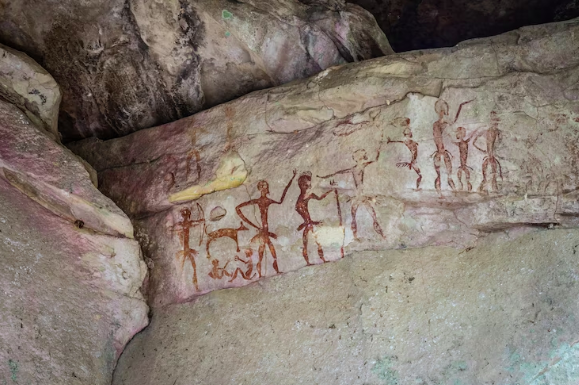
\includegraphics[width=\textwidth]{./imgs/art44.png}
\end{figure}


Assinale a alternativa que contém uma característica da manifestação representada pela imagem.

\begin{escolha}
\item
  É percebida em três dimensões: altura, profundidade e largura.
\item
  Representa as imagens em relevo.
\item
  É uma arte tridimensional de importância arqueológica.
\item
  Apresenta figuras dispostas em superfície plana.
\end{escolha}

\coment{SAEB: Reconhecer elementos constitutivos das artes visuais, dança,
música e teatro.
BNCC: EF15AR02 – Explorar e reconhecer elementos constitutivos das artes
visuais (ponto, linha, forma, cor, espaço, movimento etc.).}

\pagebreak
\num{9}  Assinale a alternativa que apresenta o nome da manifestação artística
  cujo responsável pela ação é o ator.

\begin{minipage}{.5\textwidth}
\begin{escolha}
\item
  Dança.
\item
  Escultura.
\item
  Teatro.
\item
  Artesanato.
\end{escolha}
\end{minipage}
\sidetext{SAEB: Identificar características do sistema de circulação das artes
visuais, dança, música e teatro em diferentes contextos (teatros,
palcos, museus, galerias, artistas, artesãos, curadores, produtores
etc.).
BNCC: EF15AR01 – Identificar e apreciar formas distintas das artes
visuais tradicionais e contemporâneas, cultivando a percepção, o
imaginário, a capacidade de simbolizar e o repertório imagético.}

\num{10}  Observe a imagem.

\begin{figure}[htpb!]
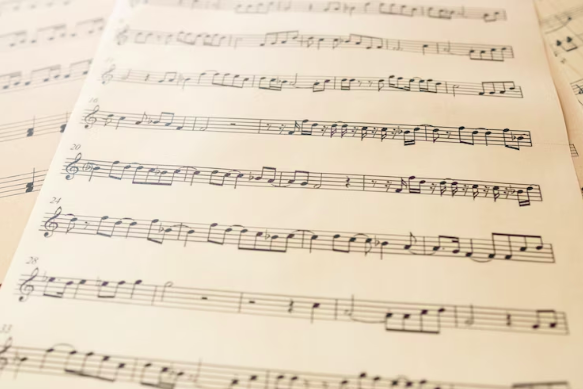
\includegraphics[width=\textwidth]{./imgs/art45.png}
\end{figure}

Na imagem, está representada

\begin{minipage}{.5\textwidth}
\begin{escolha}
\item uma obra de arte visual.
  
\item uma forma de notação musical.
  
\item um modo de apresentar um texto dramático.
  
\item um tipo de texto com linguagem verbal e não verbal.
  
\end{escolha}
\end{minipage}
\sidetext{SAEB: Reconhecer elementos constitutivos das artes visuais, dança,
música e teatro.
BNCC: EF15AR08 – Experimentar e apreciar formas distintas de
manifestações da dança presentes em diferentes contextos, cultivando a
percepção, o imaginário, a capacidade de simbolizar e o repertório
corporal.}

\pagebreak
\num{11}
Além do relógio, outro objeto que nos ajuda a contar o tempo é

%\caption{Disponível em: \emph{https://br.freepik.com/fotos-gratis/tempo-sino-acordar-branco-velho\_1044180.htm\#query=rel\%C3\%B3gio\&position=15\&from\_view=search\&track=sph} Acesso em: 23 fev. 2023.}

\begin{minipage}{0.5\textwidth}
\begin{escolha}
\item a bússola.

\item a ampulheta.

\item o termômetro.

\item a luneta.
\end{escolha}
\end{minipage}
\sidetext{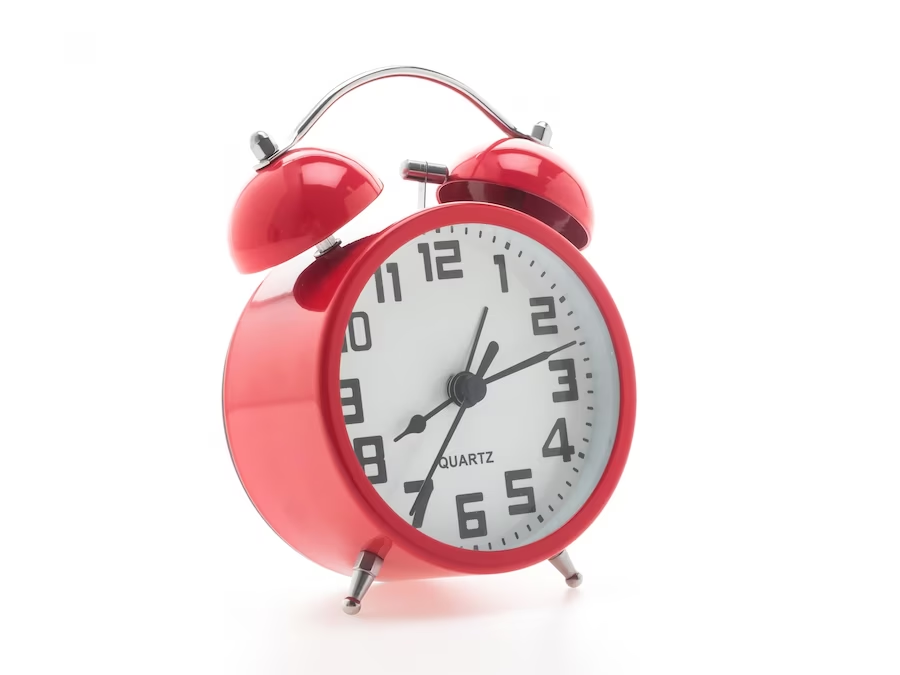
\includegraphics[width=.5\textwidth]{./imgs/img65.png}}

\coment{BNCC: EF05HI07 - Identificar os processos de produção, hierarquização e
difusão dos marcos de memória e discutir a presença e/ou a ausência de
diferentes grupos que compõem a sociedade na nomeação desses marcos de
memória.}

\num{12}

\begin{quote}
\textbf{Poluição: lixo, esgoto e metais pesados ameaçam os rios do
Brasil}

{[}\ldots{}{]}
De acordo com uma pesquisa desenvolvida pela ONG SOS Mata Atlântica, o
cenário não é nada favorável: apenas 11\% dos rios brasileiros
analisados foram considerados de boa qualidade, enquanto 35\% receberam
a classificação de “ruins” e 5\% estavam em situação crítica. O
restante, 49\%, é considerado pela organização como regular. {[}\ldots{}{]}

\fonte{Tera ambiental. Poluição: lixo, esgoto e metais pesados ameaçam os rios do Brasil. Disponível em:
\emph{https://www.teraambiental.com.br/blog-da-tera-ambiental/poluicao-lixo-esgoto-e-metais-pesados-ameacam-os-rios-do-brasil}.
Acesso em: 23 fev. 2023.}
\end{quote}

Uma atividade que pode contribuir para diminuir a poluição dos rios é

\begin{minipage}{0.5\textwidth}
\begin{escolha}
\item o desmatamento das florestas.

\item o aumento da mineração.

\item o uso de agrotóxicos.

\item a reciclagem do lixo.
\end{escolha}
\end{minipage}
\sidetext{BNCC: EF05GE10 - Reconhecer e comparar atributos da qualidade
ambiental e algumas formas de poluição dos cursos de água e dos oceanos
(esgotos, efluentes industriais, marés negras etc.).}

\pagebreak
\num{13}

\begin{figure}[htpb!]
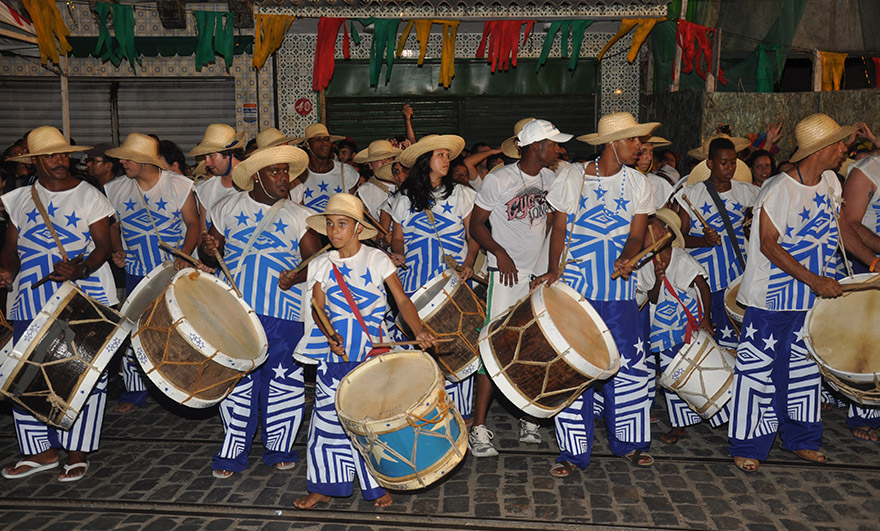
\includegraphics[width=\textwidth]{./imgs/img66.png}
\end{figure}

\begin{quote}
Maracatu Nação é um conjunto musical percussão; evoca as coroações de reis e rainhas do antigo Congo africano.
Para o Iphan, o valor desse Maracatu Nação está em sua
capacidade de comunicar elementos da cultura brasileira e carregar
elementos essenciais para memória, identidade e formação da
população afro-brasileira.

\fonte{Fonte de pesquisa:
\emph{http://portal.iphan.gov.br/pagina/detalhes/504/}
Acesso em: 23 fev. 2023.}
\end{quote}

\noindent{}O Maracatu Nação é considerado um Patrimônio Histórico Imaterial de
nosso país. Para ser considerado Patrimônio Histórico Imaterial como o
Maracatu, uma prática, um objeto, ou um saber deve

\begin{minipage}{0.5\textwidth}
\begin{escolha}
\item render dinheiro à comunidade local.

\item representar a cultura de um grupo.

\item ser praticado dentro da família.

\item ter sido criado na atualidade.
\end{escolha}
\end{minipage}
\sidetext{BNCC: EF05HI10 - Inventariar os patrimônios materiais e imateriais da
humanidade e analisar mudanças e permanências desses patrimônios ao
longo do tempo.}

\pagebreak
\num{14} O parecer CNE/CP nº 03/2004 e a Resolução CNE/CP nº 01/2004 instituem a
obrigatoriedade do ensino de História e Cultura Afro-brasileira e
Africana nos currículos das escolas da Educação
Básica. Isso se justifica pelo processo histórico de luta e
resistência dos povos negros e quilombolas.

\fonte{Fonte de pesquisa: SEDUC. Educação Escolar Quilombola. Disponível em:
\emph{https://www.seduc.ce.gov.br/educacao-escolar-quilombola/}.
Acesso em: 23 fev. 2023.}

\noindent{}Quilombolas são povos que vivem até hoje em comunidades de
afro-descendentes que combatiam a escravidão no país. A
obrigatoriedade do ensino de História e Cultura Afro-brasileira e
Africana nos currículos das escolas é importante para

\begin{escolha}
\item melhorar a qualidade das merendas escolares.

\item instituir a diversidade no ensino da cultura.

\item proteger as crianças em situação de rua.

\item garantir o fim da escravidão no Brasil.
\end{escolha}

\coment{BNCC: EF05HI04 - Associar a noção de cidadania com os
princípios de respeito à diversidade, à pluralidade e aos direitos
humanos.}

\num{15} Home Office, ao pé da letra, significa algo como “escritório em casa”. Isso significa que o
funcionário desenvolve as tarefas em sua casa, sem se
deslocar até a empresa,
utilizando principalmente a internet para se comunicar com seus colegas e chefes.

\fonte{Fonte de pesquisa:
\emph{https://www.guiadacarreira.com.br/blog/5-vantagens-de-trabalhar-em-home-office}.
Acesso em: 25 fev. 2023.}

\noindent{}Segundo o texto, hoje em dia trabalhar de casa só é possível por causa do(a)

\begin{escolha}
\item desenvolvimento das tecnologias de comunicação.

\item aumento de empregos nas indústrias de produção.

\item dificuldade de encontrar empregos presenciais.

\item criação de novas tarefas de cuidado da casa.
\end{escolha}

\coment{BNCC: EF05GE05 - Identificar e comparar as mudanças dos tipos
de trabalho e desenvolvimento tecnológico na agropecuária, na indústria,
no comércio e nos serviços.}